\chapter{Geologisk historieundersøgelse}

\textbf{NB: i det følgende kapitel skal der ses bort fra de manglende figurer og de ikke fuldstændige figur referencer.}


I dette kapitel er der en analyse af de geologiske forhold i Aalborg, samt en redegørelse for de historiske forhold der har været medvirkende til dannelse af disse geologiske forhold. 
Kapitlet vil have fokus på den glaciale, den senglaciale og den post glaciale periode, og vil yderligere også redegøre for de kridt forekomster der findes i Aalborg. 

Størstedelen af den jord der findes i Aalborg i dag, har oprindeligt været en bjergart som gennem tiden er blevet forvitret og transporteret. Det er de forskellige forhold i de forskellige tidsperioder der har været medvirkende til at de forskellige jord aflejringer er sket. Disse forskellige forhold for de forskellige perioder vil blive beskrevet herunder:

\section{Den Glaciale periode}

Glaciale perioder omfatter de perioder hvor landskabet har været dækket af gletsjere. I Danmark findes der spor efter de seneste fire istider, herunder Menap-, Elster-, Saale- og Weichsel istiden. Mellem istiderne har isen været smeltet bort, disse perioder kategoriseres som interglaciale perioder. 

Der vil i dette kapitel kun fokuseres på den sidste glaciale periode, mere specifikt Sen Weichsel perioden som strækker sig fra ca. 25.000 år siden til ca. 9.500 år siden. I denne periode var Nordjylland nedfrosset og dækket af gletsjere, disse gletsjere har medbragt nogle forvitret materialer som bl.a. omfatter forvitrede og løsrevne klippestykker fra Skandinaviens fjelde, og medslæbte bløde jordarter. Disse materiale blev under is-transporten knust og sammenblandet.

Ved isens smeltning ville dette materiale enten udfaldet som en yderest usorteret substans, eller aflejre sig som velsorterede jordarter gennem en kort/lang transport forårsaget af isens smeltevand. Denne transporten kunne have forgået under, i eller udenfor isen. 

Den usorterede blanding som er en sammenblanding af ler, sand, grus og sten, betegnes som moræne. Herfra kan man opdele det i moræneler, morænesand osv. alt efter hvad der er karakteristisk. På samme måde inddeles smeltevandsaflejringerne efter kornstørrelser

Denne transport kan ses af figur X.X 
NOTE: Johnny scanner billede fra kort  


Som det fremgår omfatter glaciale aflejringer moræneler, morænesand, morænegrus og smeltevandsaflejringer i form af smeltevandssand og –grus. 

\section{Glaciale aflejringer i Aalborgområdet}
De glaciale aflejringer kan findes flere steder i Aalborgområdet som topografisk materiale, placeringen af disse kan ses af figur X.X 
NOTE: Johnny scanner kortet for mig, det er very nice (borat stemme)

Som det ses af figur X.X findes der smeltevandssand og –grus aflejringer som topografisk materiale syd for fjorden strækkende sig fra Sønder Tranders op over Øster Sundby og videre op mod Limfjorden. Desuden findes der en større ø bestående af smeltevandssand og –grus nord for fjorden som strækker sig op til Hvorup. 

De glaciale moræner findes i et meget begrænset omfang som topografisk materiale i Aalborgområdet, der ses dog en relativt større forekomst af moræneler nær Sønder Tranders, mens de resterende forekomster af moræneler forekommer relativt sporadisk i Aalborgområdet.
 
Den sidste del af Weichsel-istiden betegnes som den senglaciale periode. Denne periode strækker sig over en periode der går fra omkring 17.000 år siden 9.500 år siden, altså frem til afslutningen af Weichsel-istiden. Denne periode markerer en overgangs periode mellem den sidste istid og den nuværende interglaciale periode. 

\section{Den senglaciale periode}
Perioden er i høj grad karakteriseret af et klima der varierede mellem tundra lignende forhold med lav vegetation, og varmere perioder med en større fauna og et rigere dyreliv. Generelt for perioden er at klimaet blev varmere hvilket betød at Nordjylland og derfor også Aalborgområdet blev isfrit da gletsjerne smeltede bort som følge af det varmere klima. Denne bortsmeltning af isen medførte markante havstigninger og betød at Nordjylland blev dækket af et ishav. Dette ishav fik navnet Yoldia havet efter en ishavsmuslingen Portlandia (tidligere Yoldia) der levede i havet. Yoldiahavets højeste strandlinjer har ligget ca. 20 m over den nuværende havoverflade, derfor vil der kunne findes senglaciale aflejringer i kote 20. De højeste strandlinjer for resten af Nordjylland ses af figur X.X


NOTE: Indsæt Yoldiakort som Johnny sama scanner for mig. 


I den nordlige del af Nordjylland hvor der var tale om havaflejringer, har området været præget af et rigt dyreliv. Her er der først blev afsat et sandlag, kaldet Nedre Saxicava-sand, som er opkaldt efter den musling som har levet i havet. Efterfølgende er der blevet afsættet er lerlag, Yoldialer, som er opkaldt efter den førnævnte Portlandia musling. Til sidst afsluttes med en sandaflejring, Øvre Saxicava-sand.

Syd for Vendsyssel, og dermed Aalborgområdet, har forholdende været anderledes. Den største forskel ligger i, at lagene ikke indeholder muslinger eller andre dyrerester. Det vil sige, at de pågældende lag ikke er blevet afsat på bunden af et hav, men er blevet opbygget i et ferskvands eller brakvandsmijø. Udover det, så er det sandlag som danner underlag for Yoldia-leret ved Vendsyssel mere sammenhængende hvorimod ved Aalborgområdet optræder sandet mere tilfældigt. Den skalfrie Yoldia-ler  som befinder sig  i Aalborgområdet har man valgt at betegne som Aalborg-ler. Som det kan ses på figur X.X, så ligger dele af Aalborg lagende forholdsvis højt. Det betyder at forekomsten af leret i Aalborg også været let tilgængelig og det har senere haft stor betydning for det lokale teglværks- og cementindustri. 

\begin{figure}[H] 
\centering
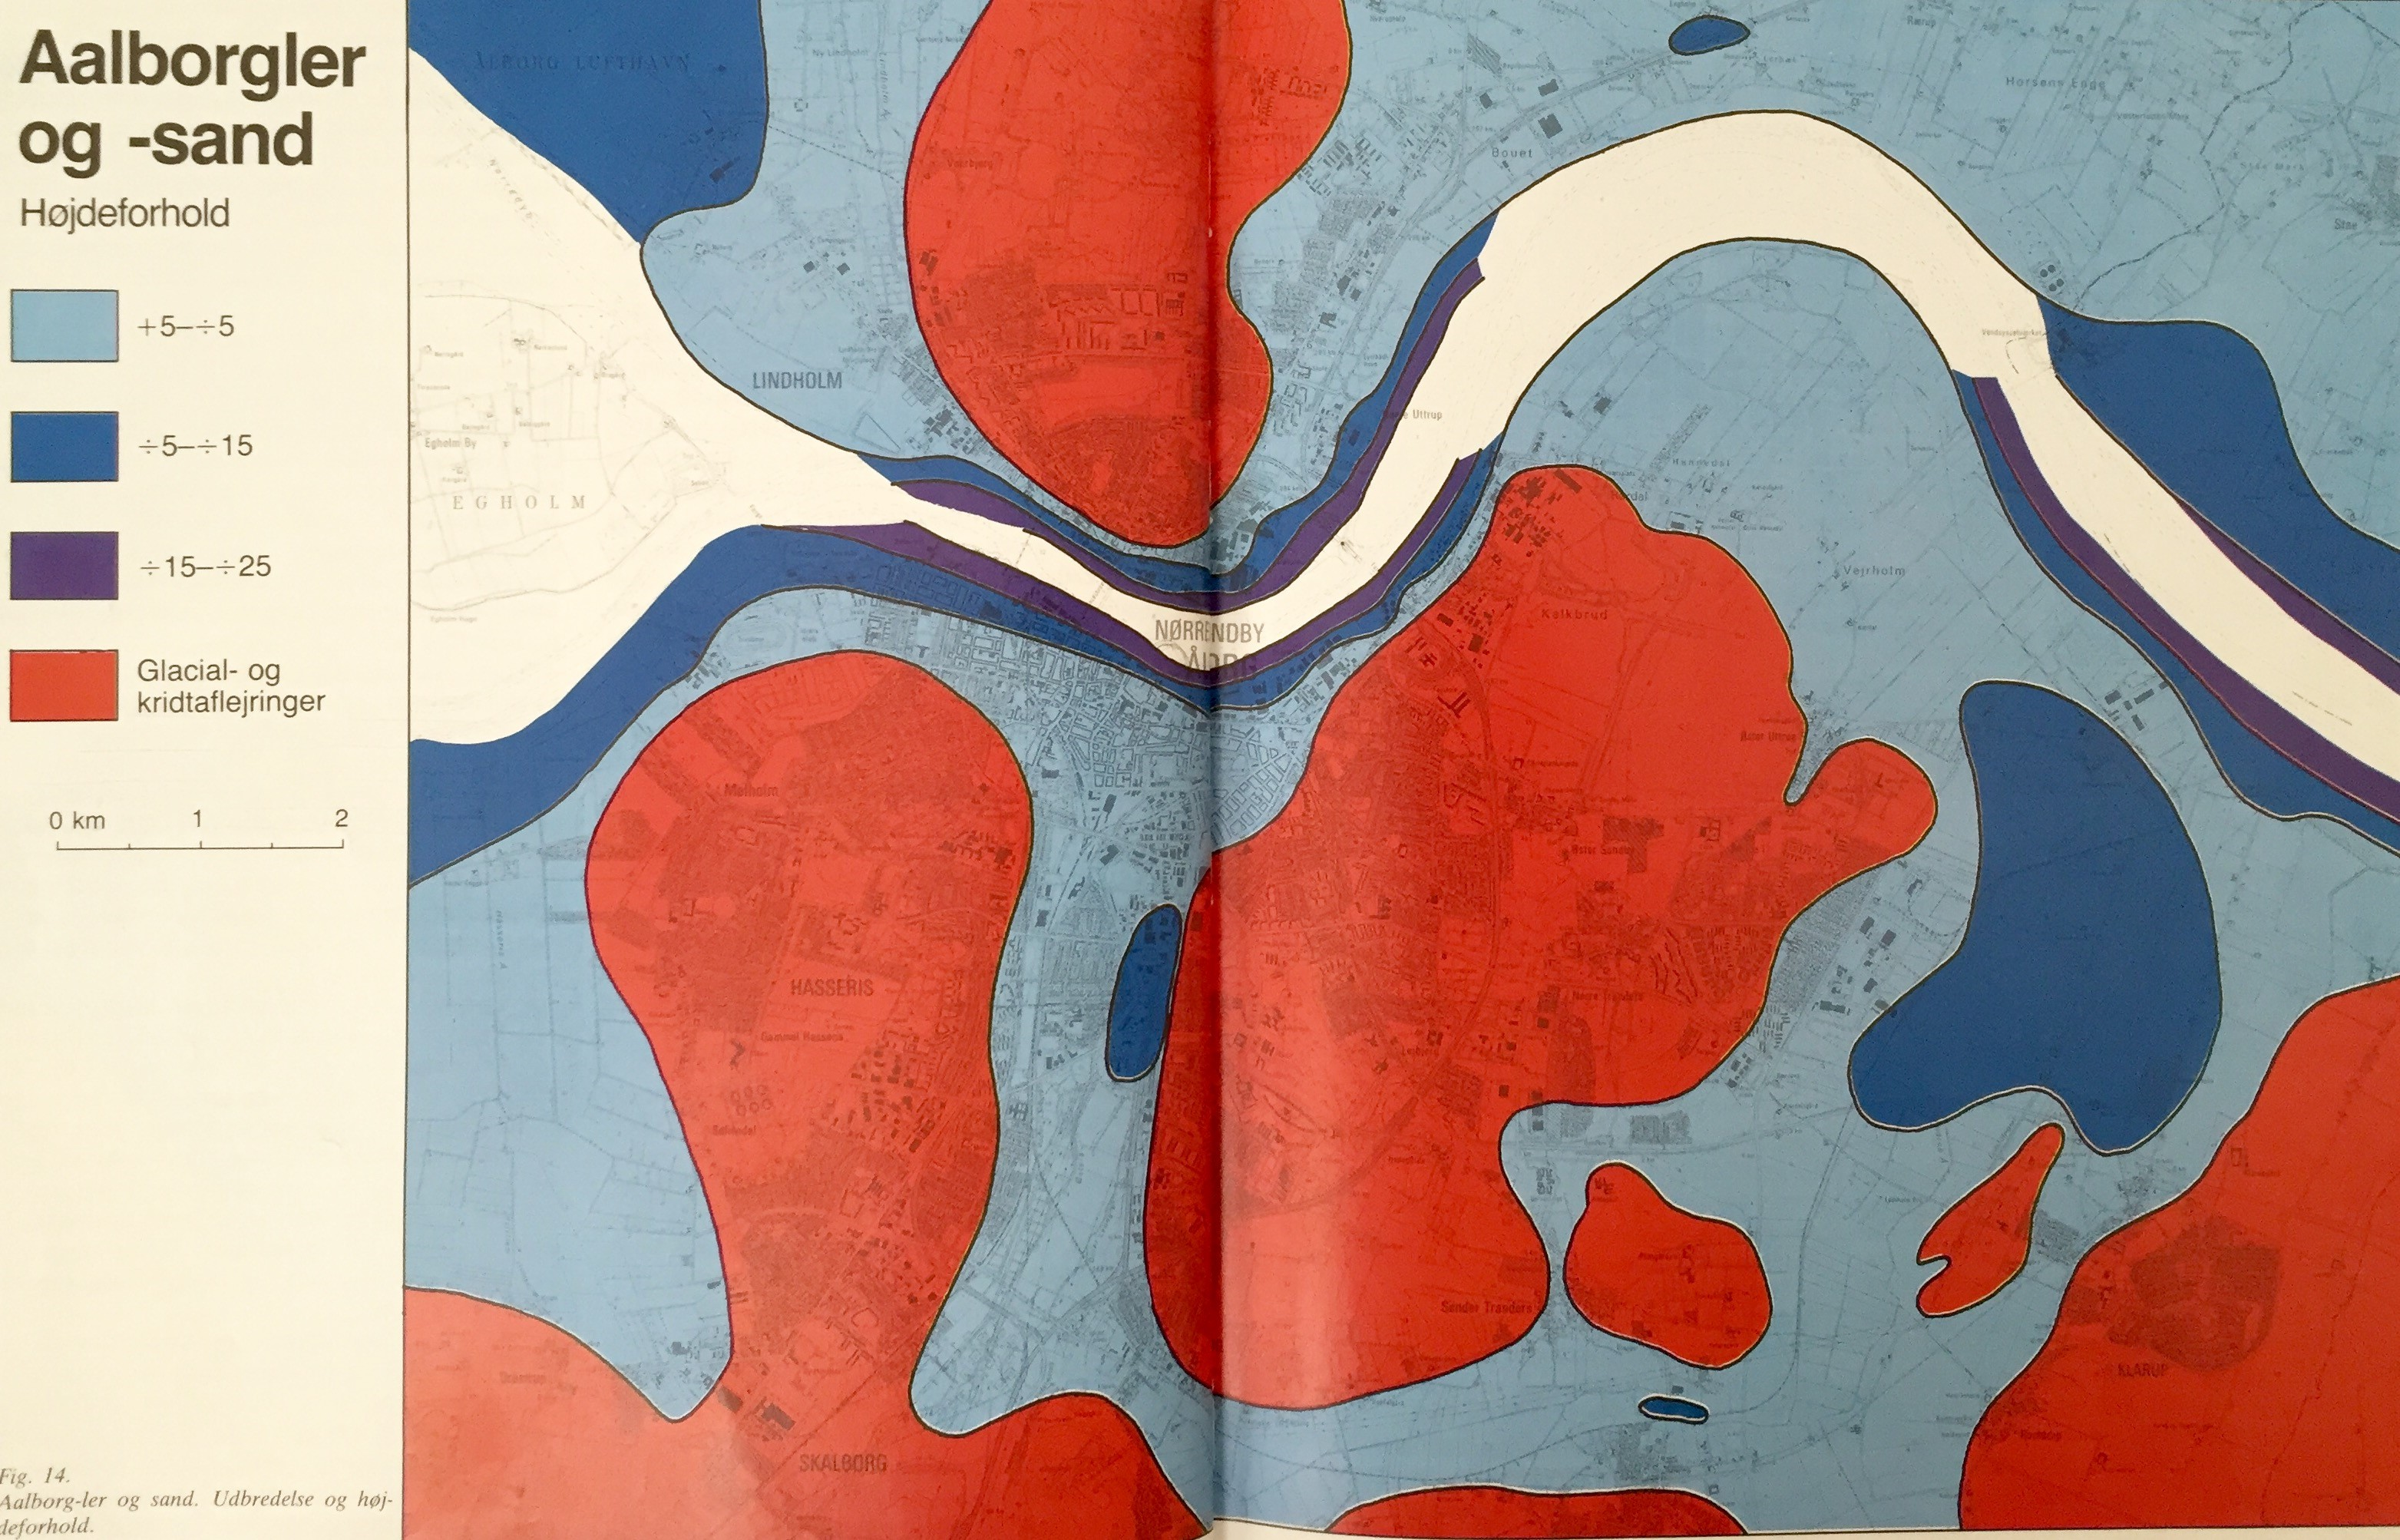
\includegraphics[width=0.90\textwidth]{billeder/GHU4}
\caption{Figuren viser forekomsterne af Aalborg-ler og -sand. Ved Limfjorden kan Aalborg-ler først findes 25 meter under fjordoverfladen.}
\label{fig:GHU4}
\end{figure}

Det ses at de senglaciale aflejringer typisk ligger lavt nær Limfjorden i Aalborg, dog ses det af Figur X.X (Det store kort med topografiske materiale) at Aalborg-leret findes som topografisk materiale i mindre områder langs Limfjordens syd- og nordlige side. 

Det ses også af kortet at det tilnærmelsesvis kan vurderes at det umiddelbare topografiske materiale der findes under Strøybergs palæ er Aalborg-ler altså en senglacial aflejring. Dette er imidlertid modstridende med den udleverede jordbundsundersøgelse, og derfor vil dette ikke blive brugt videre i rapporten. 

Efter den senglaciale periode fulgte den postglaciale periode, som startede for omkring 9.500 år siden og er endnu ikke afsluttet. Den postglaciale periode markere starten på den Holocæne epoke og Flandern – mellemistiden, som er den interglaciale periode vi i dag befinder os i. 

\section{Den Postglaciale periode}

Klimatisk set var de første ca. 2000 år af den postglaciale periode koldere end det nuværende klima, men varmere end det klima der havde domineret den senglaciale periode. For omkring 7000 år siden begyndte klimaet i højere grad at minde om det klima der ses i dag. Disse klimatiske har betydet at et stadig mere udbredte skovområder i Nordjylland, dette ses også ved at der flere steder i Aalborg er dokumenteret tørv materiale er påvist. Disse tørvforekomster ses af Figur X.X

NOTE: Scan billede på side 28 og skriv noget med at de er markeret med ringe.

De før omtale klimatiske forbedringer betød også at for omkring 7.500 år siden medførte gletsjer smeltninger i det nordlige Skandinavien at Aalborg igen var dækket af hav. Havet fik navnet Stenalderhavet da dets maksimale udbredelse lå i stenaldertiden. Der var denne gang ikke tale om et ishav, men et hav der minder meget om det der findes i Aalborg området i dag. De højeste forekommende strandlinjer for Stenalderhavet lå ca. 6-8 meter højere end det nuværende hav niveau, altså må de højeste forekommende postglaciale aflejringer forventes at kunne findes i kote 8. De resterende højeste standlinjer for Nordjylland kan ses af Figur X.X  

NOTE: Indsæt figuren fra side 47

De hyppige postglaciale aflejringer omfatter saltvandsler og saltvandssand. At den postglaciale periode er den senest forekommende periode og derfor også de senest aflejrede materialer ses også af Figur X.X (Det kvartærologiske kort) hvor af det ses at de postglaciale aflejringer er de mest udbredte topografiske materiale i Aalborg området, hvor de forekommer, både på den nordlige- , såvel som den sydlige side af Limfjorden. Det er dog værd at bemærke at manglende boringer i området umiddelbart syd for Limfjorden, betyder at dette område ikke er kortlagt. Det må dog anses som værende sandsynligt at de postglaciale aflejringer vil være hyppigt fundne som topografisk materialer i dette område. 

\section{Opsummering}

Som det ses af ovenstående kapitel findes der aflejringer fra alle tre analyserede perioder i Aalborg, både som topografisk materiale, men også dybere i jorden. I forhold til at dette projekt omhandler funderingen af tilbygning, anses det som værende relevant at se på de forskellige aflejringers egnethed som funderingsmateriale. 
Figur X.X viser et skema over de forskellige aflejringer fra de forskellige perioder, der kan findes i hele Danmark. 

NOTE: Indsæt figur fra side 43 i geobogen. Skriv figur tekst der forklare betydningen af 

Overordnet set ses det at desto ældre aflejringen er, desto bedre er styrke- og deformationsegenskaberne, og ydermere ses det også at muligheden for sætninger aftager med alderen af aflejringerne. 
Derfor ses det at de glaciale aflejringer hverken giver anledning til sætninger og har desuden styrke- og deformationsegenskaber der klassificeres som værende ”Meget gode – Gode”. Den generelle forklaring på dette, er at disse aflejringer har været hårdt sammenpresset af gletsjer masserne i de glaciale perioder og har derfor været belastet i en udstrækning der må anses som værende urealistisk at en bygning eller anden konstruktion vil nå. 

I takt med at styrke og deformationsegenskaberne falder op mod den post glaciale periode, stiger muligheden for sætninger også, og det må derfor vurderes at de post glaciale aflejringer er de mindst gunstige funderingsmateriale af de tre analyseret perioder. 

En anden bemærkelsesværdig ting der ses af figur X.X (den der står lige oven over) er det faktum at organiske aflejringer som tørv og gytje begge har ugunstige styrke- og deformationsegenskaber. En lignende udvikling ses i de faldende styrke og deformationsegenskaber fra de glaciale aflejringer til de sen glaciale aflejringer, hvor de klimatiske forbedringer, som tidligere nævnt, har givet anledning til en større fauna og et rigere dyreliv, og derfor også en øget mængde organisk materiale i periodens aflejringer generelt. 

For at sætte de forskellige perioders aflejringer i forhold til Strøybjergs Palæ, kan dette gøres med et Skematisk snit Nordjylland.


Det har ikke været muligt nøjagtigt at fastlægge koten for de glaciale aflejringer, mens at koten for både de sen glaciale aflejringer og de post glaciale aflejringer er fastlagt ud fra de tidligere benævnte maksimale strandlinjer for henholdsvis Yoldiahavet og Stenalderhavet. 
Strøybjergs Palæ ligger i Kote 2.5 og vil ud fra det ovenstående skematiske snit af Nordjylland derfor både skulle funderes i post- og sen glaciale aflejringer såvel som glaciale aflejringer. 

Med de relevante geologiske forhold i Aalborg området fastlagt er der skabt et adækvat billede den jord der skal funderes i ved opførelsen af en udbygning til Strøybergs Palæ. 

Udover at påvirke valget af funderings metode og byggeriet generelt, har de geologiske forhold i Aalborg også påvirket Aalborgs byudvikling. Udover de analyseret aflejringer fra den glaciale periode, samt den sen- og post glaciale periode, findes der i Aalborg også aflejringer af Skrivekridt der stammer tilbage fra den øvre kridttid. Disse aflejringer er flere steder højtliggende og danner tre større kridtøer. Disse kridtøer ses herunder af Figur X.X

\begin{figure}[H] 
\centering
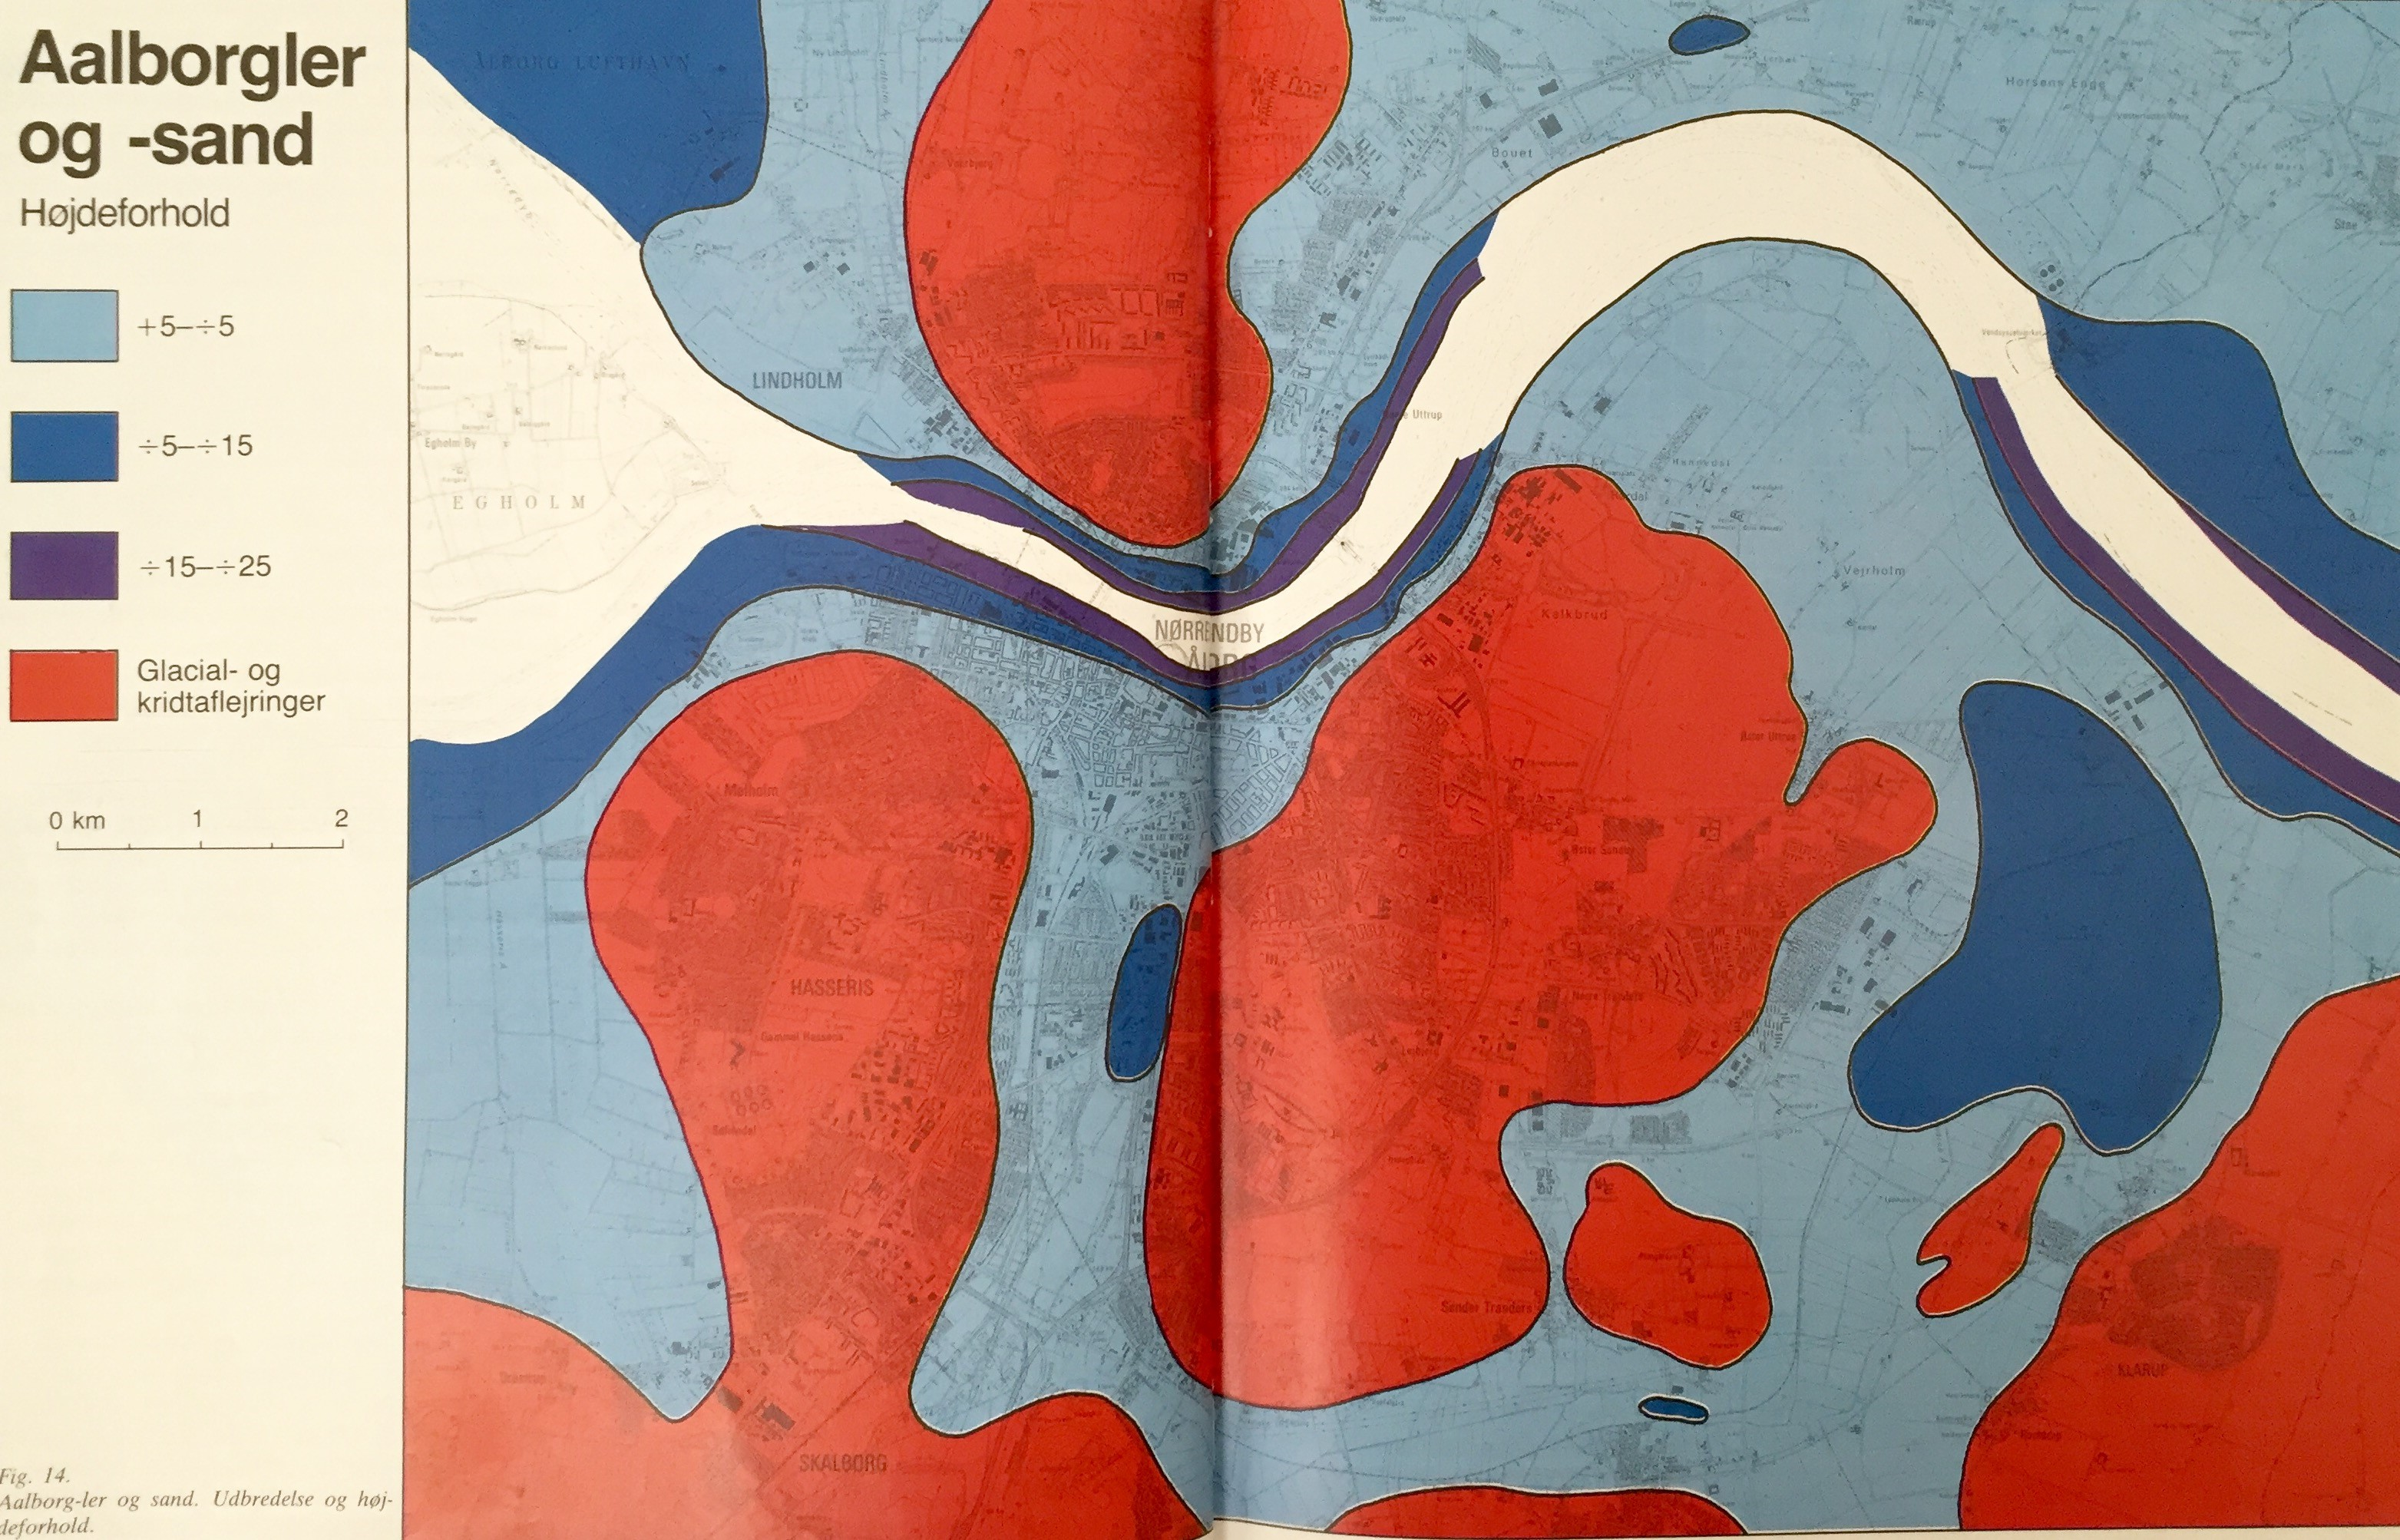
\includegraphics[width=0.90\textwidth]{billeder/GHU4}
\caption{Figuren angiver højden af kridtoverfladerne. De blåfarvede områder ligger under kote 0. De gule områder ligger højere end kote 0, og udgør de omtalte kridtøer..}
\label{fig:GHU2}
\end{figure}

Cement består af to primære komponenter, henholdsvis kalk og ler. Begge findes i jorden i Aalborg, og denne forekomst af Skrivekridt og det førnævnte Aalborg-ler har påvirket at der i den sidste del af 1800-tallet opstod en voksende cement industri i Aalborg, der i høj grad fungerede som dynamo for både byudviklingen og Aalborgs industrielle udvikling. Der findes stadig spor efter denne cement industri i Aalborg i dag i form af Aalborg Portland.

Aalborg er i dag gået fra en industriby til en kompetence by, og denne udvikling samt de visioner og nuværende tiltag Aalborg Kommune har, vil blive beskrevet og analyseret i det næste kapitel.   



